\section{Data encoding}
\par In this work, we focus on CQ, which means machine learning of classical data with quantum devices. Therefore, we need to encode the classical data into some  quantum state. A properly chosen encoding method can greatly improve the accuracy of machine learning. In quantum machine learning, sometimes encoding data is the bottleneck for the runtime of the algorithm. 

\subsection{Amplitude encoding}
\par Assume that the data $\bm{x}$ is the $2^Q$-dimensional real vector. Then, the representation of this data is the following:
$$|\psi\rangle=\sum_{k=1}^{2^Q}\frac{x_k}{\|\bm{x}\|}|k\rangle$$
where $x_k$ is the k-th element of $\bm{x}$, and $\|.\|$ is the L2-norm. The number of the required qubits is $Q$.

\par The problem of amplitude encoding is that it takes much time to prepare the quantum state. It is known that the lower bound of circuit depth for amplitude encoding is $O\left(\frac{2^Q}{Q}\right)$ for circuit with $Q$ qubits \cite{lower}. The actual algorithm currently used is worse than this and takes almost $O(2^N)$ circuit depth \cite{book1}.

\subsection{Angle encoding}
\par Assume that the data $\bm{x}$ is the $LQ$-dimensional real vector. The representation of this data is done for example by the following circuit (Figure \ref{fig:circuit5}). The number of the required qubits is $Q$. 
\begin{figure}[htb]
    \centering
    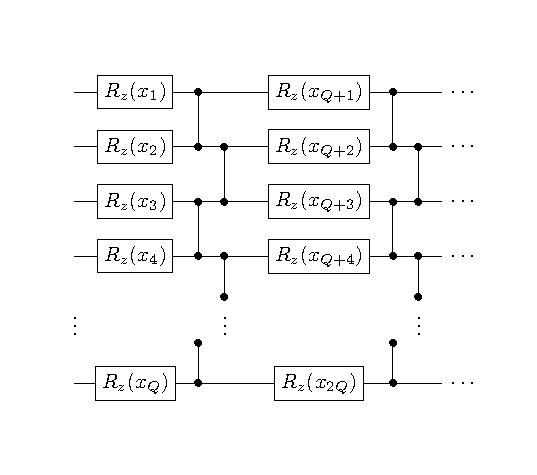
\includegraphics[keepaspectratio, scale=2]{preliminary/angle_enco.pdf}
    \caption{The example circuit of angle encoding for $LQ$-dimensional data.}
    \label{fig:circuit5}
\end{figure}

\par In this example, the first $Q$ elements are embedded into each qubit using $R_z$ gates, then these qubits are entangled using a CZ layer, and the next $Q$ elements are embedded into each qubit using fraxis gates, then entangle these qubits using a CZ layer, and so on $L$ times. Rotation operators can be $R_y$ or $R_z$. The order of data, the number of qubits, etc. can be freely determined. A method of encoding using a rotating game is called angle encoding.It is clear that the circuit depth is $O(N)$ for the data $\bm{x}\in\mathbb{R}^N$, which is far shallower than amplitude encoding.
